\chapter{Contributions}\label{chap:tra}

\section{Présentation de l'outil Acceleo}\label{sec:acc}

Acceleo est un générateur de code Open Source développé par \kwobeo{} et la fondation Eclipse.
\\
Acceleo permet de générer du code, à partir de modèles basés sur le framework EMF (\cf{} \cite{emf}), en mettant en œuvre l'approche Model Driven Architecture (MDA). Le générateur Acceleo est une implémentation de la norme de l'OMG pour les transformations de modèle vers texte (Model to Text : M2T \cf{} section \ref{sec:m2t}.

\subsection{Fonctionnement}

Comme la plupart des générateurs de code, Acceleo propose un système basé sur les templates : Les fichiers à générer peuvent être écrits avec des éléments statiques mêlés à des éléments dynamiques.

\subsubsection{Les Modules}

Dans Acceleo, un Module est une unité de génération amenée a être utilisée par le générateur. Un générateur est donc une agrégation de Modules.
\\
Un Module est paramétré par un ou plusieurs DSL (ndla : définir précédemment, a vérifier) afin de pouvoir proposer les fonctionnalités associées, qui permettent notamment de parcourir chaque élément du Modèle.
\\
Chaque Module est composée d'un ou plusieurs templates. Un template a pour rôle de générer du code d'après un ou plusieurs paramètres (éléments du Modèle). L'utilisation des templates est rendue très intuitive grâce au langage conçu pour Acceleo : Par défaut, le texte écrit dans un Template est recopié tel-quel dans le fichier qui sera généré en sortie. Afin d'insérer du contenu dynamique (base de la génération) dans le texte du Template, Acceleo utilise les balises \guim{\textbf{[}} (ouvrantes) et \guim{\textbf{/]}} (fermantes). Ces balisent permettent d'insérer un certain nombre d'instructions, comme la récupération d'un attribut d'un élément du Modèle, mais aussi des opérations conditionnelles ou des boucles de traitement.
\\
Par convention, chaque Module concerne un ou plusieurs aspects de la génération. Un Module peut également être dédié à la génération d'un type de fichier en particulier.

\begin{figure}[htb]
  \centering
  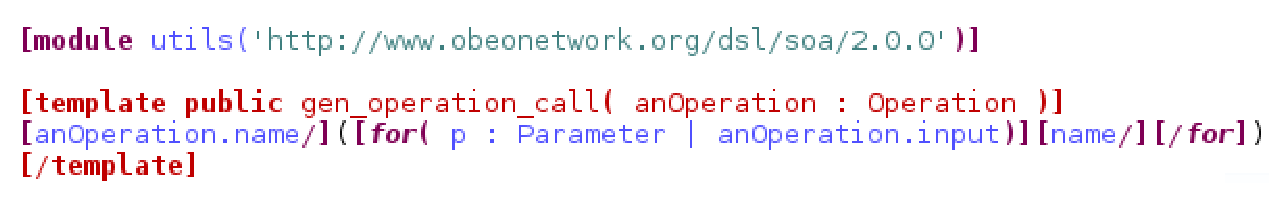
\includegraphics[scale=0.6]{img/screen_template.eps}
  \caption{Exemple de fichier Module dans Acceleo}
  \label{fig:acc_module}
\end{figure}

% Peut être une tite capture d'écran ici (Je m'en charge)

\subsubsection{Les Queries}

Les Modules permettent de décomposer la génération du code en plusieurs sous-parties réutilisables. Ils sont donc utiles pour générer un même type de contenu texte à partir de différents éléments du même type.\\
Cependant, dans certains cas, il est nécessaire d'exécuter une opération sur un élément du Modèle, comme la modification d'une chaine, ou l'accès à l'élément parent d'un élément, par exemple.\\
Les Queries interviennent alors comme un moyen de déporter ces opérations non-triviales dans une base commune. Les spécificité des Queries par rapport aux templates est que ces dernières mettent en cache leur résultat. Ainsi, si une Query est appelée deux fois avec les mêmes paramètres, celle-ci ne sera pas re-calculée et se contentera de retourner le résultat obtenu précédement. Cette fonctionnalité est donc très utile pour l'appel répétitif d'opérations (même basiques), ou le stockage de variables globales.\\
Les Queries permettent plus généralement de structure le générateur. Par convention, les générations de texte sont traitées dans des templates, tandis que les opérations plus complexes (modification de chaine, parcours d'éléments) ou répétitive sont déportées dans des Queries.

\begin{figure}[htb]
  \centering
  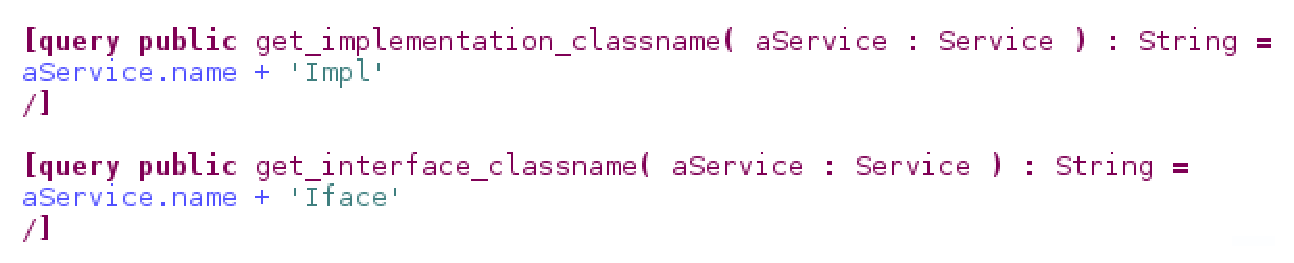
\includegraphics[scale=0.6]{img/screen_query.eps}
  \caption{Exemple de Queries dans Acceleo}
  \label{fig:acc_module}
\end{figure}

\subsubsection{Les Services}

Les Services peuvent être vus comme une extension des Queries. Là où les opérations exécutables des Query se limitent à celles d'Ocl (TODO : Aborder Ocl). Le principe des Services consiste à appeler du code Java depuis une Query via des invocations de méthodes. Cela permet d'effectuer des opérations complexes ou bien de stocker un certain nombre d'informations via du code Java. Ces informations restent récupérables depuis les templates pendant toute la durée de la génération de code.

\subsubsection{Les balises \guim{Code Utilisateur}}

Si un Générateur de Code permet aisément de transcrire la structure et la logique de fonctionnement d'un système, il est en revanche impossible d'en saisir automatiquement tous les aspects ou particularités. En d'autres termes, un code généré sera rarement complet. \kwacceleo fournit donc un système très simple permettant de définir des zones de \guim{Code Utilisateur} au sein d'un Template. Ainsi, l'utilisateur peut apporter des modifications ou ajouts dans les fichiers générés. Si ces modifications ont été effectuées à l'intérieur d'une zone \guim{Code Utilisateur}, ces dernières ne seront pas affectées si les fichiers sont générés à nouveau. De telles zones peuvent être insérée au sein d'un Template en utilisant de simples balises \guim{\textit{\textbf{[protected]}}}

% Ici un schema ?
\begin{figure}[htb]
  \centering
  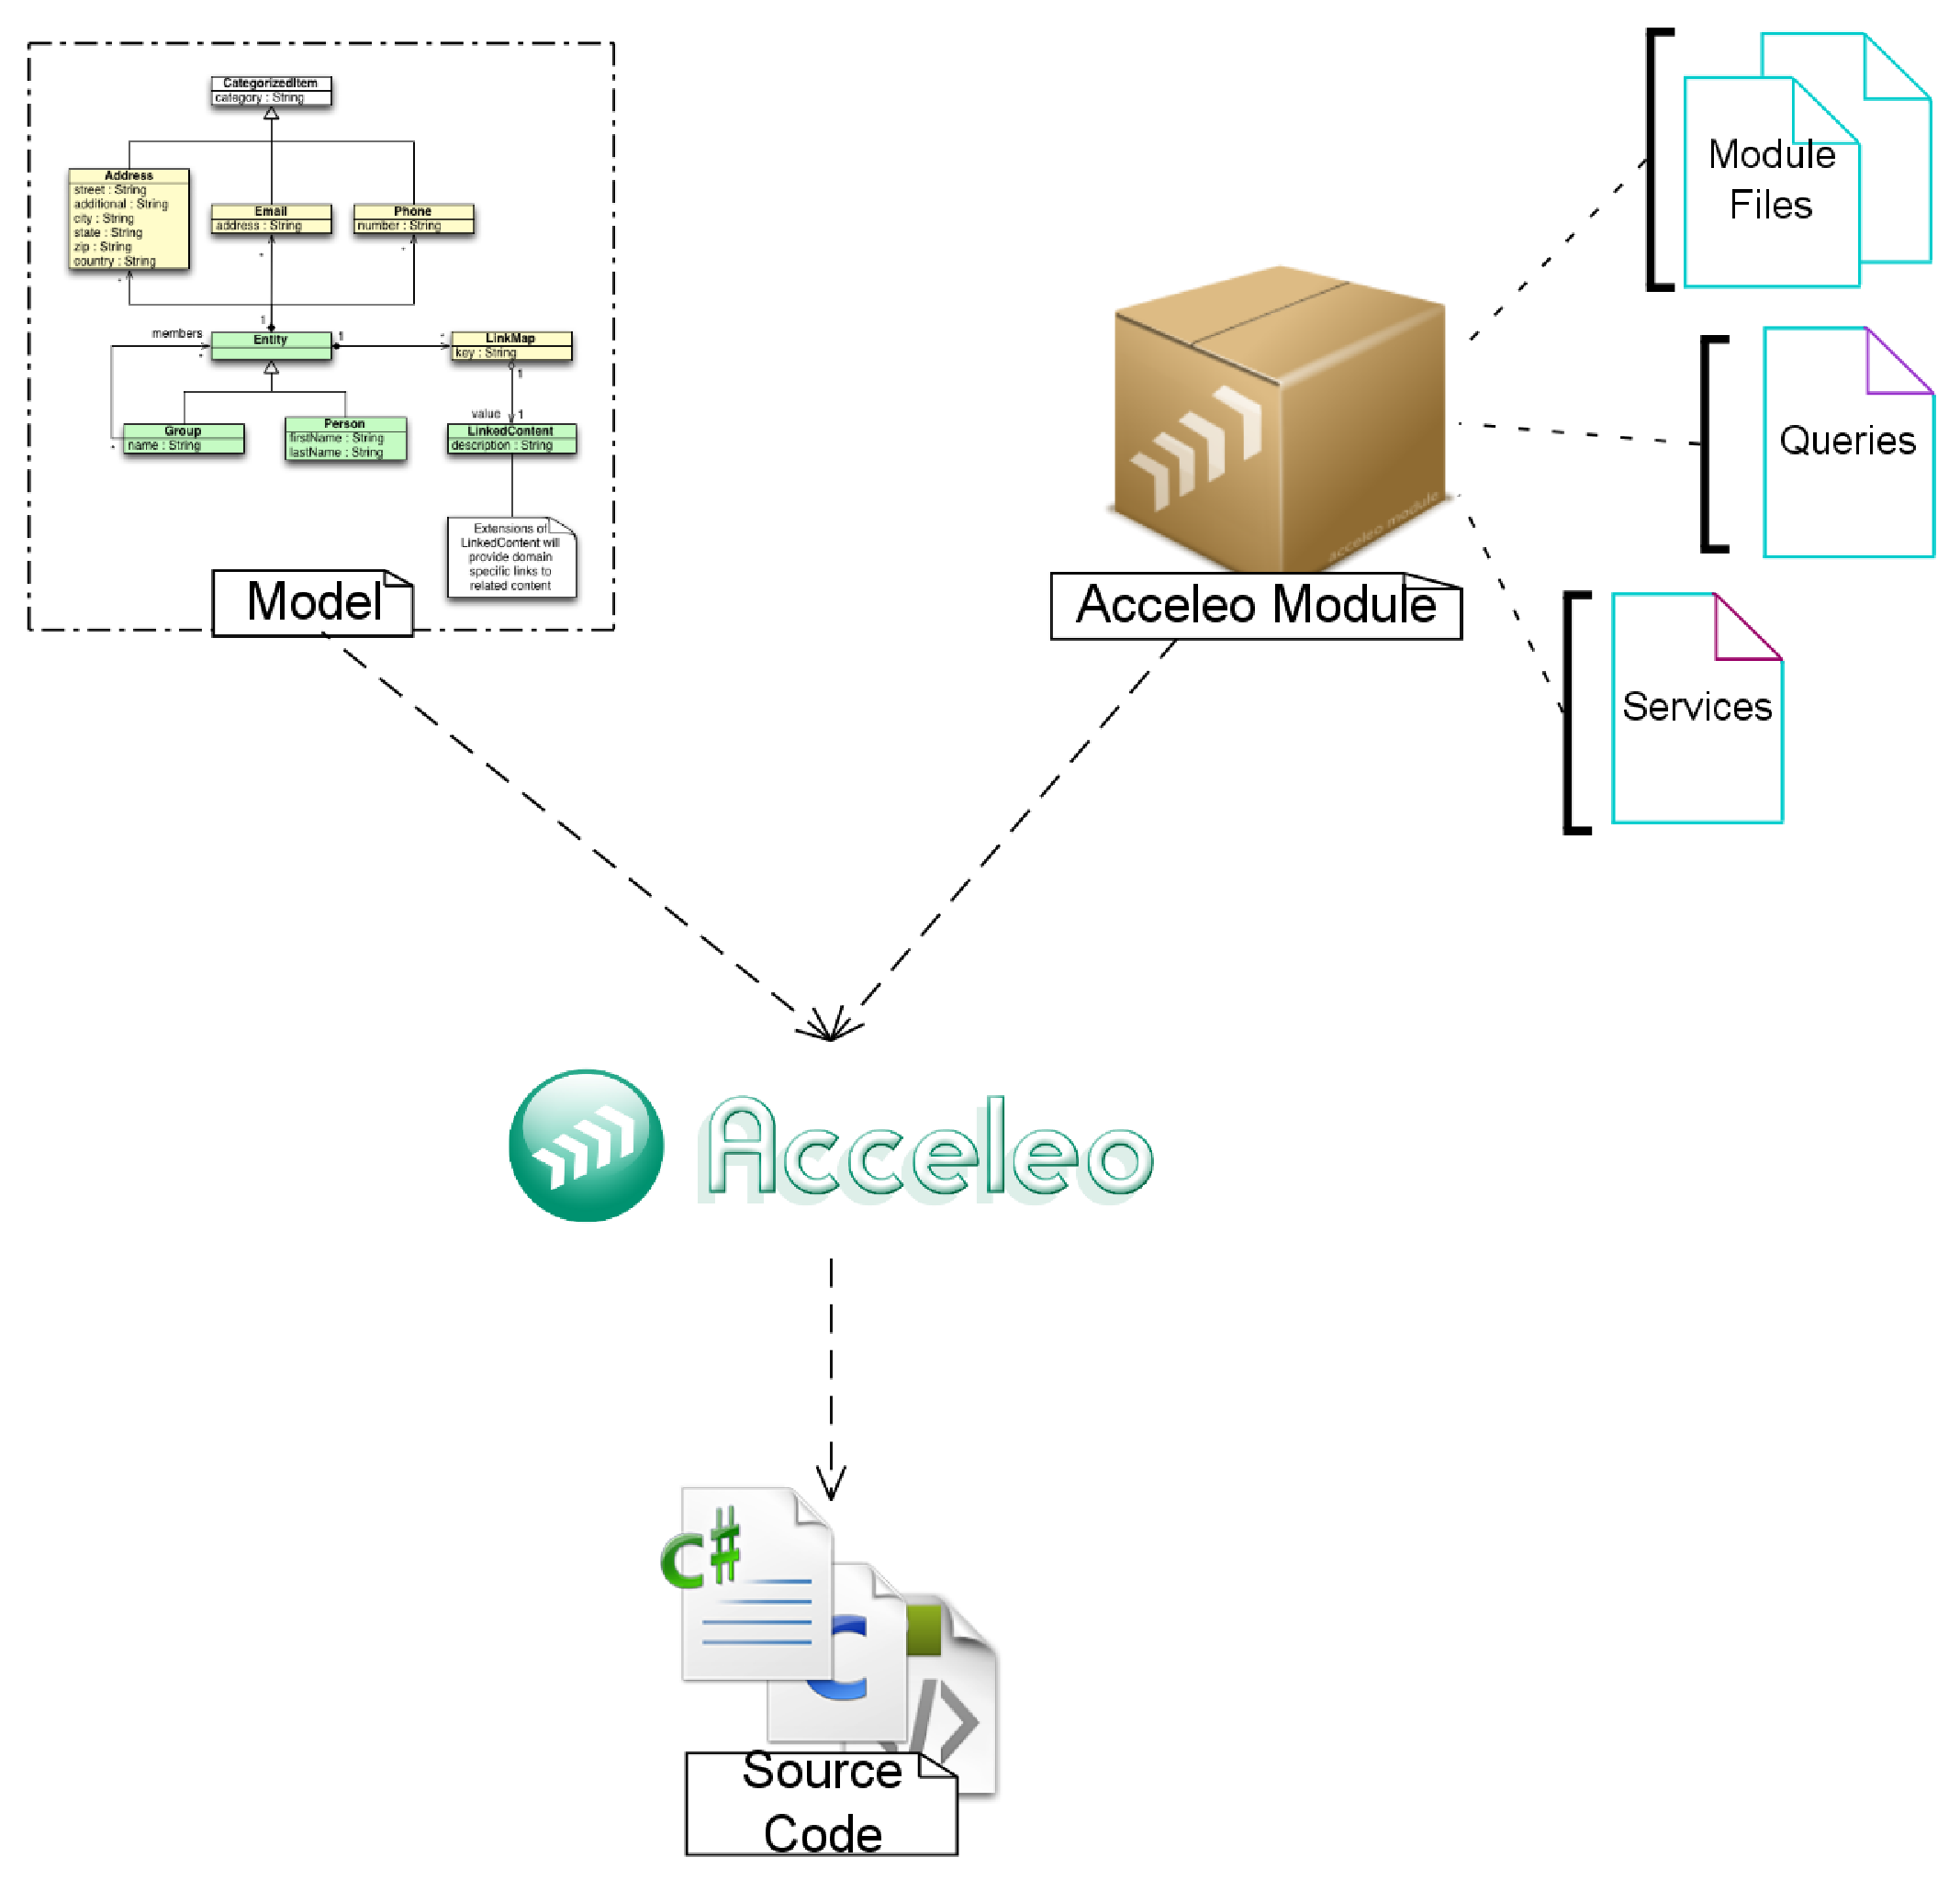
\includegraphics[scale=0.29]{img/acceleo_scheme.eps}
  \caption{Fonctionnement d'Acceleo}
  \label{fig:acceleo}
\end{figure}

%\subsection{Déploiement}
%
%Afin de gérer le déploiement des différents générateurs de %code, 

% Causer du système de menus/plugins/etc

\newpage

\section{Le Méta-Modèle Entity}\label{sub:ent}


Le méta-modèle \kwentity{} représente une couche \og métier \fg{}. Il permet notamment de modéliser la persistance des données, ainsi que les relations entres elles. La figure \ref{fig:ent}  montre le méta-modèle Entity simplifié.

\begin{figure}[H]
  \centering
  
\includegraphics[scale=.4]{img/Entity.eps}
  \caption{Méta-modèle Entity}
  \label{fig:ent}
\end{figure}

Chaque block se compose de plusieurs Entity. Celle-ci possède un ou plusieurs attributs, et peut référencer d'autres Entity. Un attribut peut avoir une métadonnée qui peut être constituée d'une ou plusieurs annotations.   

\subsection{Gestion des entités avec \kwplay{}}

Dans la plate-forme Play, tout le code métier est porté par les objets du modèle. Celui-ci contient les données persistantes, ce qui s'accordent parfaitement avec le concept d'\kwentity.  
%% On peut par exemple écrire le code suivant pour manipuler une entité "Personne" :\\
         
%% \fbox{\parbox{\textwidth}{
%% // Si on voulait récupérer toutes les personnes    \\
%% List<Personne> personnes = Personne.find("byName","Takfarinas").fetch();  \\
%% Personne p1 = Personne.findById(1);  // Récupérer la personne ayant l'id 1  \\
%% p1.firstName = "paul";  // Modification de l'entité  \\
%% p1.save(); // Mise à jour dans la base de données  

%% }}
%% \\
%% \\
\subsection{Conception du modèle}
Nous avons employé la simple démarche suivante : pour chaque module Play, on associe une entité. À ce stade, on en déduit facilement les attributs de chaque instance d'\verb+Entity+ et les instances \verb+Reference+ correspondant aux associations avec d'autres entités. \kwplay{} utilise des mécanismes d'annotation au sein de ses modèles. Ces annotations permettent notamment de donner des contraintes à des attributs. Nous avons facilement pris en compte ce concept en utilisant la classe \verb+Annotation+ mise à disposition dans les méta datas d'un \verb+Attribut+.

Nous avons élaboré un modèle d'Entity de notre application conformément au Méta-Modèle que nous avons décris précédement. Ce modèle est illustré par la figure \ref{fig:entMod} ci-dessous.

\begin{figure}[H]
  \centering
  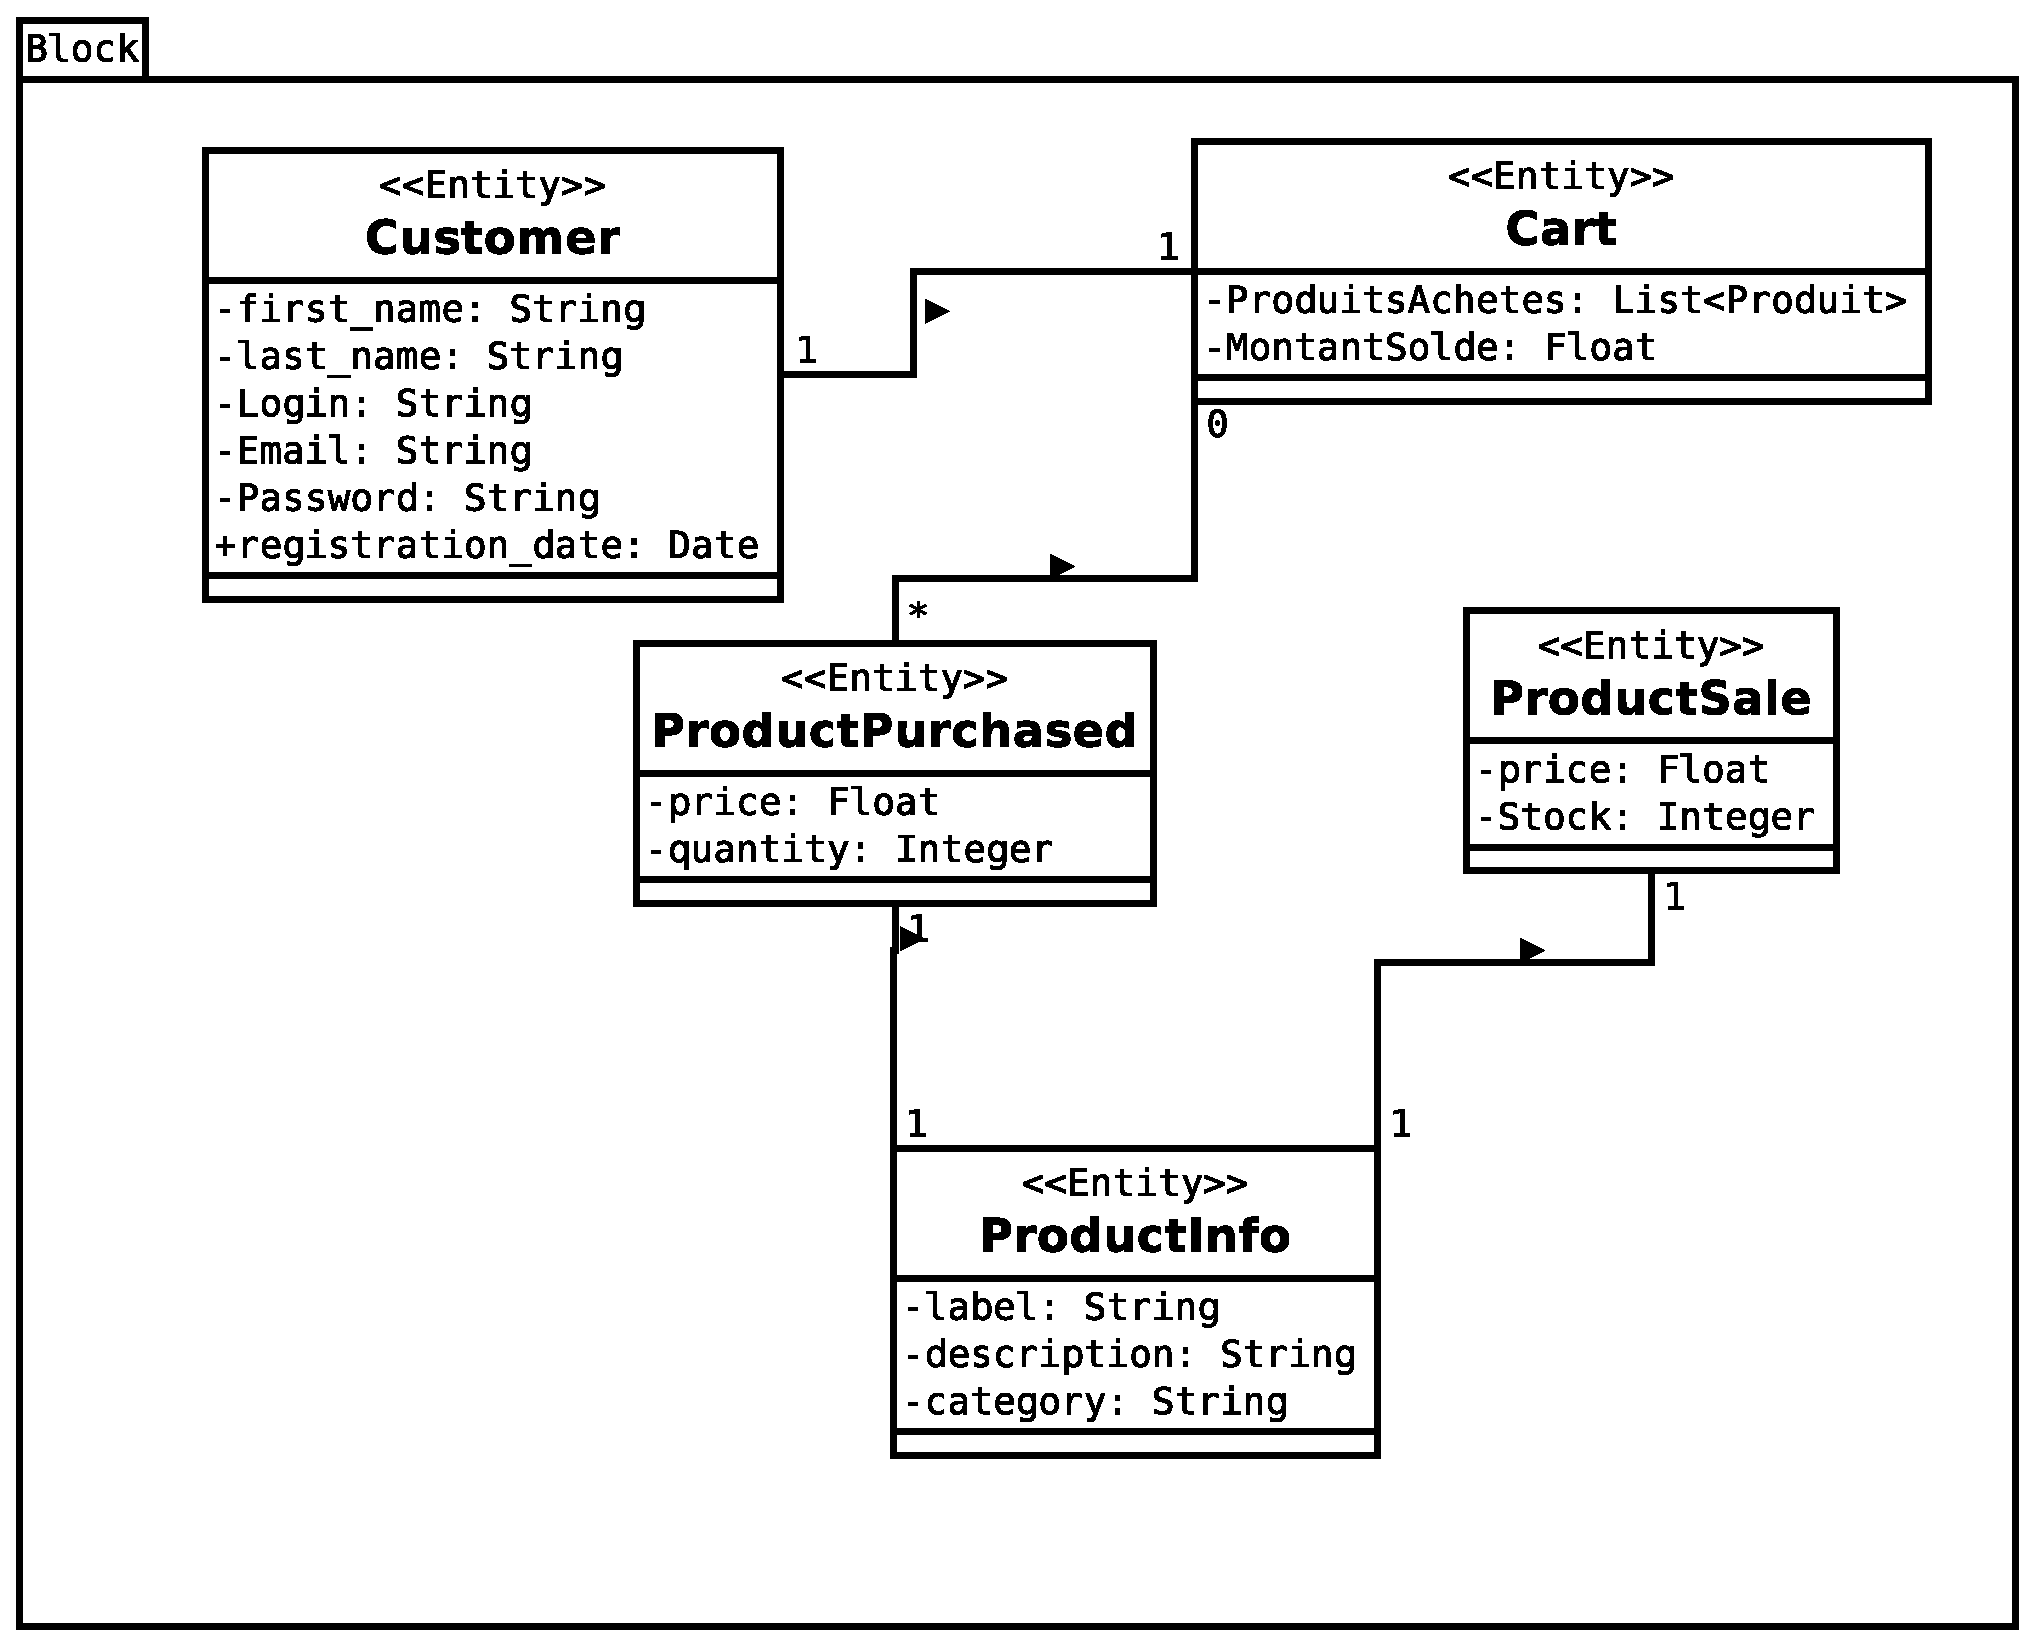
\includegraphics[scale=.4]{img/Entitymodel.eps}
  \caption{modèle Entity de l'application}
  \label{fig:entMod}
\end{figure}

Nous avons représenté un seul bloque dans notre modèle d'Entity qui va regrouper les Entity suivantes :  

\begin{itemize}
  \item[\textbullet] \textbf{Customer} :  client qui va faire l'achat sur la plate-forme.
  \item[\textbullet] \textbf{ProductSale} : les produits mis en vente.
  \item[\textbullet] \textbf{ProductPurchased} : les produits achetés par un client.
  \item[\textbullet] \textbf{ProductInfo} : contient les informations d'un produit.
  \item[\textbullet] \textbf{Cart} : panier virtuel du client.
\end{itemize}

\subsection{Génération du code Entity}

L'étape de construction des Générateurs de Code pour le Modèle \kwentity a été relativement simple : Pour chaque \kwentity contenue dans le Modèle, on crée génère une simple classe Java portant le nom de ladite Entité, puis on liste l'ensemble de ses attributs (types et propriétés). Ainsi, l'ORM \kwebean (intégré à \kwplay) interprétera simplement ces classes comme étant des données à stocker dans une Base.


%% \fbox{\parbox{\textwidth}{
%% [template public generateElement(myBlock : Block)]   // création du template.\newline
%% [for( myEntity : Entity | myBlock.entities)] //parcours des Entity. \newline
%% [file (myEntity.name + g-name-suffix() + '.java', false, 'UTF-8')] //création d'un fichier.\newline
%% [for(myEntity.attributes)] // parcours de tout les attributs. 
%% 	[comment Call the file block in 'attributes' /]\newline
%% 	[ generateAttribute() /] // appel d'un autre template qui affiche les attributs.\newline
%% [/for]
%% }}



% LocalWords:  Entity framework Model
 
\section{\kwsoa}\label{sub:soa}

\kwsoa (Service Oriented Architecture) - ou Architecture Orientée Services - modélise le concept de Services et d'Opérations au travers d'un système basé sur les Composants. Concrêtement, un modèle basé sur \kwsoa est constitué de Composants. Chaque Composant peut possèder des Services dont des Interfaces permettent de communiquer avec l'extérieur. Ces Interfaces définissent une une plusieurs Opérations, chaque opération étant caractérisée par un ensemble de Paramètres d'entrée et de sortie. Ces paramètres peuvent être des types relativement basiques (Integer, String, ...) mais également des \guim{Entity} complexes, comme des informations complètes sur les utilisateurs, ou sur des produits.	

\begin{figure}[htb]
  \centering
  
\includegraphics[scale=.3]{img/SOA.eps}
  \caption{Métamodèle SOA}
  \label{fig:soa}
\end{figure}

\subsection{Le concept de \kwsoa{} dans \kwplay{}}

\kwplay{}, de part son achitecture en MVC, ne propose pas d'implémentation concrête de la notion de Services. 
Nous avons donc fait le choix de déporter ces derniers dans des classes externes de type Singleton, ce qui permet de faire appel aux différents Services depuis n'importe quel Controleur de \kwplay{}. (\textit{Services.getAKindOfService().do\_service()}). 
Cela permet de séparer les différents concepts sans pour autant remettre en cause l'architecture originelle de \kwplay{}.

\subsection{Conception du modèle}

La conception du modèle SOA pour le contexte de notre magasin en ligne a été assez simple à convenir : Pour chaque cas d'utilisation ou action, nous avons modélisé un certain nombre d'opérations basiques. Ces opérations ont été réunies dans différents Composants et Services, en fonction de leur contexte, mais également en fonction du type d'utilisateur susceptible de faire appel à ces opérations.\\
Ainsi, les opérations consistant à inscrire ou connecter un utilisateur ont été regroupées au sein d'un \textit{AuthentificationManager} accessible uniquement par l'application en elle-même. 

\subsection{Génération du code des services}

\subsubsection{Séparation interfaces/implémentations}

Afin d'assurer une souplesse de l'application, la génération des différents Services systématiquement découpée en deux parties :
\begin{itemize}
\item Des interfaces, contenant les signatures des différentes opérations.
\item Des classes d'implémentation, liées à ces interfaces.
\end{itemize}	

Les classes d'implémentation sont générées avec le code des différentes opérations, lorsque celles-ci sont basiques et/ou facilement interprêtables (récupérer/éditer/détruire une entité). Dans tous les cas, des balises \guim{user code} (à définir) sont également insérées afin de laisser libre choix à l'utilisateur pour les détails de l'implémentation.\\
Cette séparation interfaces/implémentations permet également d'avoir plusieurs types d'implémentation de Services pour une même interface.\\
Nous avons implémenté les différentes classes de Services comme étant des Singleton. Il est ainsi possible d'appeler un Service depuis n'importe quel endroit de l'application avec une syntaxe du type \textit{Services.getMonPremierService().faireMonTravail()}.

\subsubsection{Plus loin avec SOA : Les webservices}

Ils nous a été proposé d'ajouter des couches supplémentaires par dessus les simples implémentations de Services SOA, notamment au niveau des moyens d'accéder à ces Services.\\
Nous avons donc mis en place des solutions permettant d'appeler certains Services depuis l'extérieur, sans passer par l'interface du site Web. Pour ce faire, nous avons procédé à la mise en place d'un service de type REST (REpresentational State Transfer).\\
Le principe est de recevoir des requêtes HTTP de type GET/POST/PUT/DELETE provenant d'autres programme que des simples navigateurs. \\
Par exemple, il devrait être possible d'appeler certains services depuis un logiciel de gestion, pour la gestion des ventes des produits, des factures, ou des comptes utilisateurs, ou pour collecter des informations.
\\\\
Nous avons donc implémenté un tel système, en configurant - pour chaque opération accessible depuis l'extérieur - des Routes spécifiques, déclenchant l'exécution des opération, et retournant un résultat au format \textit{JSON}.

\clearpage

\section{Cinématique}
\subsection{Modélisation}
\subsubsection{Vue globale du métamodèle}
Le métamodèle est organisé autour de trois principaux packages:
\begin{itemize}
  \item View: représente les concepts liés à la définition des écrans IHM.
Le package View est construit de la manière suivante:
\newline
-> insérer viewDiagramme
  \item Toolkit: représente les concepts liés à la définition des
  widgets\footnote{Elément visuel d'une interface graphique (bouton, ascenseur,
  liste déroulante, etc.)} IHM.
Le package Toolkit est construit de la manière suivante:
\newline
-> insérer toolkitDiagramme
  \item Flow: permet d'identifier le comportement dynamique des écrans IHM.
  Le flow peut être appréhendé comme une sorte de diagramme d'activités.
Le package Flow est construit de la manière suivante:
\newline
-> insérer flowDiagramme
\end{itemize}

\subsubsection{Le modèle}

****************Description du modèle***************

\subsection{Le générateur}
\subsubsection{Organisation et généricité ?}
\subsubsection{}
\subsection{Résultats obtenus}

\inputnp{4d_Deploiement}
